\documentclass[a4paper,14pt,oneside,openany]{memoir}

%%% Задаем поля, отступы и межстрочный интервал %%%

\usepackage[left=30mm, right=15mm, top=20mm, bottom=20mm]{geometry} % Пакет geometry с аргументами для определения полей
\pagestyle{plain} % Убираем стандарные для данного класса верхние колонтитулы с заголовком текущей главы, оставляем только номер страницы снизу по центру
\parindent=1.25cm % Абзацный отступ 1.25 см, приблизительно равно пяти знакам, как по ГОСТ
\usepackage{indentfirst} % Добавляем отступ к первому абзацу
%\linespread{1.3} % Межстрочный интервал (наиболее близко к вордовскому полуторному) - тут вместо этого используется команда OnehalfSpacing*

%%% Задаем языковые параметры и шрифт %%%

\usepackage[english, russian]{babel}                % Настройки для русского языка как основного в тексте
\babelfont[russian]{rm}{Times New Roman}                     % TMR в качестве базового roman-щрифта



%%% Задаем стиль заголовков и подзаголовков в тексте %%%

\setsecnumdepth{subsection} % Номера разделов считать до третьего уровня включительно, т.е. нумеруются только главы, секции, подсекции
\renewcommand*{\chapterheadstart}{} % Переопределяем команду, задающую отступ над заголовком, чтобы отступа не было
\renewcommand*{\printchaptername}{} % Переопределяем команду, печатающую слово "Глава", чтобы оно не печалось
%\renewcommand*{\printchapternum}{} % То же самое для номера главы - тут не надо, номер главы оставляем
\renewcommand*{\chapnumfont}{\normalfont\bfseries} % Меняем стиль шрифта для номера главы: нормальный размер, полужирный
\renewcommand*{\afterchapternum}{\hspace{1em}} % Меняем разделитель между номером главы и названием
\renewcommand*{\printchaptertitle}{\normalfont\bfseries\centering\MakeUppercase} % Меняем стиль написания для заголовка главы: нормальный размер, полужирный, центрированный, заглавными буквами
\setbeforesecskip{20pt} % Задаем отступ перед заголовком секции
\setaftersecskip{20pt} % Ставим такой же отступ после заголовка секции
\setsecheadstyle{\raggedright\normalfont\bfseries} % Меняем стиль написания для заголовка секции: выравнивание по правому краю без переносов, нормальный размер, полужирный
\setbeforesubsecskip{20pt} % Задаем отступ перед заголовком подсекции
\setaftersubsecskip{20pt} % Ставим такой же отступ после заголовка подсекции
\setsubsecheadstyle{\raggedright\normalfont\bfseries}  % Меняем стиль написания для заголовка подсекции: выравнивание по правому краю без переносов, нормальный размер, полужирный

%%% Задаем параметры оглавления %%%

\addto\captionsrussian{\renewcommand\contentsname{Содержание}} % Меняем слово "Оглавление" на "Содержание"
\setrmarg{2.55em plus1fil} % Запрещаем переносы слов в оглавлении
%\setlength{\cftbeforechapterskip}{0pt} % Эта команда убирает интервал между заголовками глав - тут не надо, так красивее смотрится
\renewcommand{\aftertoctitle}{\afterchaptertitle \vspace{-\cftbeforechapterskip}} % Делаем отступ между словом "Содержание" и первой строкой таким же, как у заголовков глав
%\renewcommand*{\chapternumberline}[1]{} % Делаем так, чтобы номер главы не печатался - тут не надо
\renewcommand*{\cftchapternumwidth}{1.5em} % Ставим подходящий по размеру разделитель между номером главы и самим заголовком
\renewcommand*{\cftchapterfont}{\normalfont\MakeUppercase} % Названия глав обычным шрифтом заглавными буквами
\renewcommand*{\cftchapterpagefont}{\normalfont} % Номера страниц обычным шрифтом
\renewcommand*{\cftchapterdotsep}{\cftdotsep} % Делаем точки до номера страницы после названий глав
\renewcommand*{\cftdotsep}{1} % Задаем расстояние между точками
\renewcommand*{\cftchapterleader}{\cftdotfill{\cftchapterdotsep}} % Делаем точки стандартной формы (по умолчанию они "жирные")
\maxtocdepth{subsection} % В оглавление попадают только разделы первыхтрех уровней: главы, секции и подсекции

%%% Выравнивание и переносы %%%

%% http://tex.stackexchange.com/questions/241343/what-is-the-meaning-of-fussy-sloppy-emergencystretch-tolerance-hbadness
%% http://www.latex-community.org/forum/viewtopic.php?p=70342#p70342
\tolerance 1414
\hbadness 1414
\emergencystretch 1.5em                             % В случае проблем регулировать в первую очередь
\hfuzz 0.3pt
\vfuzz \hfuzz
%\dbottom
%\sloppy                                            % Избавляемся от переполнений
\clubpenalty=10000                                  % Запрещаем разрыв страницы после первой строки абзаца
\widowpenalty=10000                                 % Запрещаем разрыв страницы после последней строки абзаца
\brokenpenalty=4991                                 % Ограничение на разрыв страницы, если строка заканчивается переносом

%%% Объясняем компилятору, какие буквы русского алфавита можно использовать в перечислениях (подрисунках и нумерованных списках) %%%
%%% По ГОСТ нельзя использовать буквы ё, з, й, о, ч, ь, ы, ъ %%%
%%% Здесь также переопределены заглавные буквы, хотя в принципе они в документе не используются %%%

\makeatletter
    \def\russian@Alph#1{\ifcase#1\or
       А\or Б\or В\or Г\or Д\or Е\or Ж\or
       И\or К\or Л\or М\or Н\or
       П\or Р\or С\or Т\or У\or Ф\or Х\or
       Ц\or Ш\or Щ\or Э\or Ю\or Я\else\xpg@ill@value{#1}{russian@Alph}\fi}
    \def\russian@alph#1{\ifcase#1\or
       а\or б\or в\or г\or д\or е\or ж\or
       и\or к\or л\or м\or н\or
       п\or р\or с\or т\or у\or ф\or х\or
       ц\or ш\or щ\or э\or ю\or я\else\xpg@ill@value{#1}{russian@alph}\fi}
\makeatother

%%% Задаем параметры оформления рисунков и таблиц %%%

\usepackage{graphicx, caption, subcaption} % Подгружаем пакеты для работы с графикой и настройки подписей
\graphicspath{{images/}} % Определяем папку с рисунками
\captionsetup[figure]{font=small, width=\textwidth, name=Рисунок, justification=centering} % Задаем параметры подписей к рисункам: маленький шрифт (в данном случае 12pt), ширина равна ширине текста, полнотекстовая надпись "Рисунок", выравнивание по центру
\captionsetup[subfigure]{font=small} % Индексы подрисунков а), б) и так далее тоже шрифтом 12pt (по умолчанию делает еще меньше)
\captionsetup[table]{singlelinecheck=false,font=small,width=\textwidth,justification=justified} % Задаем параметры подписей к таблицам: запрещаем переносы, маленький шрифт (в данном случае 12pt), ширина равна ширине текста, выравнивание по ширине
\captiondelim{ --- } % Разделителем между номером рисунка/таблицы и текстом в подписи является длинное тире
\setkeys{Gin}{width=\textwidth} % По умолчанию размер всех добавляемых рисунков будет подгоняться под ширину текста
\renewcommand{\thesubfigure}{\asbuk{subfigure}} % Нумерация подрисунков строчными буквами кириллицы
%\setlength{\abovecaptionskip}{0pt} % Отбивка над подписью - тут не меняем
%\setlength{\belowcaptionskip}{0pt} % Отбивка под подписью - тут не меняем
\usepackage[section]{placeins} % Объекты типа float (рисунки/таблицы) не вылезают за границы секциии, в которой они объявлены

%%% Задаем параметры ссылок и гиперссылок %%% 

\usepackage{hyperref}                               % Подгружаем нужный пакет
\hypersetup{
    colorlinks=true,                                % Все ссылки и гиперссылки цветные
    linktoc=all,                                    % В оглавлении ссылки подключатся для всех отображаемых уровней
    linktocpage=true,                               % Ссылка - только номер страницы, а не весь заголовок (так выглядит аккуратнее)
    linkcolor=red,                                  % Цвет ссылок и гиперссылок - красный
    citecolor=red                                   % Цвет цитировний - красный
}

%%% Настраиваем отображение списков %%%

\usepackage{enumitem}                               % Подгружаем пакет для гибкой настройки списков
\renewcommand*{\labelitemi}{\normalfont{--}}        % В ненумерованных списках для пунктов используем короткое тире
\makeatletter
    \AddEnumerateCounter{\asbuk}{\russian@alph}     % Объясняем пакету enumitem, как использовать asbuk
\makeatother
\renewcommand{\labelenumii}{\asbuk{enumii})}        % Кириллица для второго уровня нумерации
\renewcommand{\labelenumiii}{\arabic{enumiii})}     % Арабские цифры для третьего уровня нумерации
\setlist{noitemsep, leftmargin=*}                   % Убираем интервалы между пунками одного уровня в списке
\setlist[1]{labelindent=\parindent}                 % Отступ у пунктов списка равен абзацному отступу
\setlist[2]{leftmargin=\parindent}                  % Плюс еще один такой же отступ для следующего уровня
\setlist[3]{leftmargin=\parindent}                  % И еще один для третьего уровня

%%% Счетчики для нумерации объектов %%%

\counterwithout{figure}{chapter}                    % Сквозная нумерация рисунков по документу
\counterwithout{equation}{chapter}                  % Сквозная нумерация математических выражений по документу
\counterwithout{table}{chapter}                     % Сквозная нумерация таблиц по документу

%%% Реализация библиографии пакетами biblatex и biblatex-gost с использованием движка biber %%%

\usepackage{csquotes} % Пакет для оформления сложных блоков цитирования (biblatex рекомендует его подключать)
\usepackage[%
backend=biber,                                      % Движок
bibencoding=utf8,                                   % Кодировка bib-файла
sorting=none,                                       % Настройка сортировки списка литературы
style=gost-numeric,                                 % Стиль цитирования и библиографии по ГОСТ
language=auto,                                      % Язык для каждой библиографической записи задается отдельно
autolang=other,                                     % Поддержка многоязычной библиографии
sortcites=true,                                     % Если в квадратных скобках несколько ссылок, то отображаться будут отсортированно
movenames=false,                                    % Не перемещать имена, они всегда в начале библиографической записи
maxnames=5,                                         % Максимальное отображаемое число авторов
minnames=3,                                         % До скольки сокращать число авторов, если их больше максимума
doi=false,                                          % Не отображать ссылки на DOI
isbn=false,                                         % Не показывать ISBN, ISSN, ISRN
]{biblatex}[2016/09/17]
\DeclareDelimFormat{bibinitdelim}{}                 % Убираем пробел между инициалами (Иванов И.И. вместо Иванов И. И.)
\addbibresource{bibl.bib}                           % Определяем файл с библиографией

%%% Скрипт, который автоматически подбирает язык (и, следовательно, формат) для каждой библиографической записи %%%
%%% Если в названии работы есть кириллица - меняем значение поля langid на russian %%%
%%% Все оставшиеся пустые места в поле langid заменяем на english %%%

\DeclareSourcemap{
  \maps[datatype=bibtex]{
    \map{
        \step[fieldsource=title, match=\regexp{^\P{Cyrillic}*\p{Cyrillic}.*}, final]
        \step[fieldset=langid, fieldvalue={russian}]
    }
    \map{
        \step[fieldset=langid, fieldvalue={english}]
    }
  }
}

%%% Прочие пакеты для расширения функционала %%%

\usepackage{longtable,ltcaption}                    % Длинные таблицы
\usepackage{multirow,makecell}                      % Улучшенное форматирование таблиц
\usepackage{booktabs}                               % Еще один пакет для красивых таблиц
\usepackage{soulutf8}                               % Поддержка переносоустойчивых подчёркиваний и зачёркиваний
\usepackage{icomma}                                 % Запятая в десятичных дробях
\usepackage{hyphenat}                               % Для красивых переносов
\usepackage{textcomp}                               % Поддержка "сложных" печатных символов типа значков иены, копирайта и т.д.
\usepackage[version=4]{mhchem}                      % Красивые химические уравнения
\usepackage{amsmath}                                % Усовершенствование отображения математических выражений 

%%% Вставляем по очереди все содержательные части документа %%%

\begin{document}

\thispagestyle{empty}

\begin{center}
    МИНИСТЕРСТВО ЦИФРОВОГО РАЗВИТИЯ, СВЯЗИ И МАССОВЫХ КОММУНИКАЦИЙ \\ РОССИЙСКОЙ ФЕДЕРАЦИИ

    \vspace{20pt}

    Федеральное государственное бюджетное образовательное учреждение  \\  высшего образования \\
    "<Сибирский государственный университет телекоммуникаций и информатики"> \\

    \vspace{20pt}

    Кафедра телекоммуникационных систем и вычислительных средств \\  (ТС и ВС)
\end{center}

\vfill

\begin{center}
    РЕФЕРАТ \\  
    по дисциплине \\
    \textit{"<Моделирование мобильных систем">}

    \vspace{20pt}

    по теме: \\
    \uppercase{ИМИТАЦИОННАЯ МОДЕЛЬ КАНАЛА СВЯЗИ OFDM В MATLAB}
\end{center}

\vfill

    \noindent Студент: \\
    \textit{Группа № ИА-232 \hfill К.К Ошлаков}

    \vspace{20pt}

    \noindent Предподаватель: \\
    \textit{должность, уч. степень, уч. звание \hfill Р.В. Ахпашев}

\vfill

\begin{center}
    Новосибирск 2025 г.
\end{center}                                     % Титульник

\newpage % Переходим на новую страницу
\setcounter{page}{2} % Начинаем считать номера страниц со второй
\OnehalfSpacing* % Задаем полуторный интервал текста (в титульнике одинарный, поэтому команда стоит после него)

\tableofcontents*                                   % Автособираемое оглавление

\chapter*{Введение}
\addcontentsline{toc}{chapter}{Введение}
\label{ch:intro}

Развитие современных систем связи требует постоянного совершенствования методов передачи информации для обеспечения высокой надежности, эффективности и устойчивости к помехам. Особую роль играют технологии цифровой обработки сигналов, позволяющие реализовать сложные алгоритмы кодирования, модуляции, эквалайзирования и демодуляции.

В рамках данного цикла практических работ проводится комплексное исследование и реализация основных функциональных блоков системы цифровой связи с использованием программной среды MATLAB. Целью работы является изучение принципов построения современных систем связи, а также получение практических навыков по реализации ключевых алгоритмов обработки сигналов.

В ходе выполнения практических работ будут последовательно реализованы и исследованы следующие компоненты: знаковое кодирование и декодирование, помехоустойчивое кодирование (сверточное кодирование и декодирование Витерби), перемежение битовой последовательности, QPSK модуляция, OFDM модуляция, модель канала передачи с замираниями и аддитивным белым гауссовским шумом, а также приемная часть системы, включающая эквалайзирование и OFDM демодуляцию. Завершающий этап работы посвящен анализу производительности реализованной системы путем расчета коэффициента битовых ошибок (BER) и построения графиков.

Каждая практическая работа включает в себя теоретическое описание реализуемого блока, детализацию его программной реализации на языке MATLAB, демонстрацию результатов тестирования в виде консольного вывода и, при необходимости, графических представлений.

Полученные в результате работы знания и навыки будут способствовать пониманию принципов функционирования современных цифровых систем связи и станут основой для дальнейшего изучения и разработки более сложных телекоммуникационных систем.

\endinput                                     % Введение
% \chapter{Знаковое кодирование}

\section{Введение}

Знаковое кодирование представляет собой метод представления текстовой информации в двоичном формате. Основная цель этой практической работы – реализовать процесс кодирования и декодирования текстового сообщения, используя заданный алфавит и разрядность кодового слова.

\section{Описание знакового кодера}

Знаковый кодер предназначен для преобразования входного символьного сообщения в последовательность двоичных символов (бит). Исходное сообщение состоит из латинских букв (маленьких и заглавных), цифр (0–9), пробела и точки, всего 64 символа.

\subsection{Принцип работы кодера}

Каждому символу входного сообщения присваивается уникальный двоичный код.

Количество бит для кодирования одного символа определяется разрядностью кодового слова.

Итоговое битовое сообщение формируется путем последовательного соединения кодов всех символов исходного текста.

\subsection{Описание входных и выходных данных}

Входные данные: текстовое сообщение длиной от 30 до 100 символов.

Выходные данные: битовая последовательность, представляющая закодированное сообщение.

\section{Описание знакового декодера}

Знаковый декодер выполняет обратную операцию: преобразует битовую последовательность обратно в текстовое сообщение. Для этого используется та же знаковая кодировка, что и в кодере.

\subsection{Принцип работы декодера}

Битовое сообщение разделяется на фрагменты, соответствующие длине кодового слова.

Каждому фрагменту сопоставляется соответствующий символ из заданного алфавита.

Восстанавливается исходное текстовое сообщение.

\subsection{Описание входных и выходных данных}

Входные данные: битовая последовательность.

Выходные данные: исходное текстовое сообщение.

\section{Выводы}

В данной работе был рассмотрен процесс знакового кодирования и декодирования текстового сообщения. Реализованный кодер позволяет эффективно преобразовывать текст в битовую форму, а декодер успешно восстанавливает исходные данные. Этот метод широко применяется в системах обработки и хранения информации.                                     % Первая глава
% \chapter{Формирование и передача OFDM сигнала}

\section{Практика 5. OFDM модуляция}

\subsection{Описание}
Пятая практическая работа посвящена реализации модуляции по принципу OFDM (Orthogonal Frequency-Division Multiplexing - ортогональное частотное мультиплексирование). OFDM является широко используемым методом модуляции в современных системах связи благодаря своей устойчивости к многолучевому распространению и интерференции.

\subsection{Реализация}
Был разработан OFDM модулятор (\texttt{ofdm\_modulator.m}) со следующими ключевыми компонентами:
\begin{itemize}
    \item \textbf{Вставка пилотных символов}: В сигнал добавляются известные пилотные символы для последующей оценки канала.
    \item \textbf{Добавление нулевых поднесущих}: Добавляются нулевые поднесущие по краям спектра для обеспечения защиты от внеполосных излучений и облегчения фильтрации.
    \item \textbf{Применение ОБПФ}: Выполняется обратное быстрое преобразование Фурье для формирования временного OFDM символа.
    \item \textbf{Добавление циклического префикса}: В начало OFDM символа добавляется копия его конца для борьбы с межсимвольной интерференцией.
\end{itemize}
Параметры модуляции, такие как интервал пилотных символов ($\Delta R_s$), длина циклического префикса ($T_{CP}$), процент нулевых поднесущих ($C$) и общее число поднесущих ($N_{subcarrier}$), сохраняются для использования в демодуляторе.

\subsection{Результаты тестирования}
В данной практической работе производится только модуляция, без обратного преобразования. Проверка корректности производится на последующих этапах, когда сигнал пройдет через канал и будет демодулирован. Консольный вывод показывает фрагмент сгенерированного OFDM символа.

\begin{verbatim}
% START - TASK: 5
disp('TASK 5: ');

delta_Rs = 6;
T_CP = 16;
C = 0.25;
N_subcarrier = 128;

ofdm_symbol = ofdm_modulator(modulatedSymbols, delta_Rs, T_CP, C, N_subcarrier);

% disp(ofdm_symbol) % Полный вывод закомментирован в коде

% END - TASK: 5
\end{verbatim}

\subsection{Консольный вывод}
\begin{verbatim}
TASK 5:
\end{verbatim}
(Консольный вывод для этой задачи пустой, так как \texttt{disp(ofdm\_symbol)} закомментировано)

\section{Практика 6. Модель канала передачи}

\subsection{Описание}
Шестая практическая работа посвящена реализации модели канала передачи с учетом замираний и аддитивного белого гауссовского шума (АБГШ). Реалистичная модель канала необходима для оценки производительности системы связи в условиях, приближенных к реальным.

\subsection{Реализация}
Была реализована функция \texttt{channel\_model.m}, моделирующая канал со следующими характеристиками:
\begin{itemize}
    \item \textbf{Многолучевое распространение}: Сигнал достигает приемника по нескольким путям ($N_b$ лучей) с разными задержками и ослаблениями.
    \item \textbf{Случайные задержки лучей}: Задержки для каждого луча генерируются случайным образом.
    \item \textbf{Добавление АБГШ}: К сигналу примешивается аддитивный белый гауссовский шум с заданной мощностью ($N_0$), определяемой отношением сигнал/шум (SNR).
\end{itemize}
Модель канала принимает на вход OFDM символ и возвращает принятый сигнал, прошедший через канал.

\subsection{Результаты тестирования}
Работа модели канала была проверена путем пропускания OFDM символа, сгенерированного на предыдущем этапе, через модель. Консольный вывод показывает фрагмент принятого сигнала.

\begin{verbatim}
% START - TASK: 6
disp('TASK 6: ');

N_path = 3;
N0_dB = 15;
max_delay = 6;
rx_signal = channel_model(ofdm_symbol, N_path, N0_dB, max_delay);

disp(rx_signal); % Отображение полного сигнала
% END - TASK: 6
\end{verbatim}

\subsection{Консольный вывод}
\begin{verbatim}
TASK 6:
  Columns 1 through 13

   1.3812 - 0.8223i   0.0111 - 0.1080i  -1.0138 + 0.7830i ... (фрагмент)

  Columns 14 through 26

   0.7438 - 1.3265i  -3.3089 + 0.5977i   1.1598 + 0.3892i ... (фрагмент)

  Columns ... (и так далее для всех столбцов)

   ...  0.0007 + 0.0138i
\end{verbatim}
Принятый сигнал представляет собой комплексные значения, которые включают в себя искажения от канала и шум. В документе представлен только фрагмент для наглядности.

\section{Практика 7. Эквалайзирование и OFDM демодуляция}

\subsection{Описание}
Седьмая практическая работа посвящена реализации приемной части системы связи, включающей OFDM демодуляцию и эквалайзирование. Эти этапы позволяют восстановить исходные символы из принятого OFDM сигнала, прошедшего через канал.

\subsection{Реализация}
Был разработан OFDM демодулятор (\texttt{ofdm\_demodulator.m}), выполняющий следующие действия:
\begin{itemize}
    \item \textbf{Удаление циклического префикса}: Удаляется добавленный на передаче циклический префикс.
    \item \textbf{БПФ}: Выполняется быстрое преобразование Фурье для перехода из временной области в частотную.
    \item \textbf{Оценка канала по пилотным символам}: Используются принятые пилотные символы для оценки частотной характеристики канала.
    \item \textbf{Эквалайзирование}: Выполняется компенсация искажений, внесенных каналом, на основе оценки канала.
    \item \textbf{Удаление нулевых поднесущих}: Удаляются нулевые поднесущие, добавленные на передаче.
\end{itemize}
Полученные в результате демодуляции символы (QPSK символы) далее передаются на демодулятор QPSK.

\subsection{Результаты тестирования}
Корректность работы OFDM демодулятора и эквалайзера оценивается на следующем этапе, где происходит демодуляция полученных символов и декодирование битовой последовательности.

\begin{verbatim}
% START - TASK: 7

disp('TASK 7: ');

received_symbols = ofdm_demodulator(rx_signal, delta_Rs, T_CP, C, N_subcarrier);
% received_symbols = ofdm_demodulator(ofdm_symbol, delta_Rs, T_CP, C, N_subcarrier);
demodulatedBits = qpsk_demodulator(received_symbols);

% disp('Original QPSK symbols:'); % Полный вывод закомментирован
% disp(modulatedSymbols);
% disp('Received QPSK symbols:'); % Полный вывод закомментирован
% disp(received_symbols);

% END - TASK: 7
\end{verbatim}

\subsection{Консольный вывод}
\begin{verbatim}
TASK 7:
\end{verbatim}
(Консольный вывод для этой задачи пустой)

\section{Практика 8. Расчет характеристик и построение графиков}

\subsection{Описание}
Восьмая практическая работа посвящена анализу производительности разработанной системы связи путем расчета коэффициента битовых ошибок (BER) и построения графиков, иллюстрирующих спектр сигналов и сигнальные созвездия.

\subsection{Реализация}
\subsubsection{Расчет BER}
Производится сравнение принятой и демодулированной битовой последовательности с исходной битовой последовательностью, полученной после перемежения. Подсчитывается количество ошибочных битов и вычисляется BER как отношение количества ошибок к общему числу переданных битов.

\subsubsection{Построение графиков}
Строятся следующие графики:
\begin{itemize}
    \item Спектр переданного OFDM символа.
    \item Спектр принятого OFDM символа (до эквалайзирования).
    \item Сигнальное созвездие QPSK символов в передатчике.
    \item Сигнальное созвездие QPSK символов в приемнике (после OFDM демодуляции и эквалайзирования).
\end{itemize}
Эти графики позволяют визуально оценить влияние канала на сигнал и эффективность эквалайзирования.

\subsection{Результаты тестирования}
Ниже представлены консольный вывод с рассчитанным BER и сгенерированные графики.

\begin{verbatim}
% START - TASK: 8
disp('TASK 8: ');

min_length = min(length(demodulatedBits), length(interleavedBits));

demodulatedBits_truncated = demodulatedBits(1:min_length);
interleavedBits_truncated = interleavedBits(1:min_length);

% Расчет BER
bit_errors = sum(demodulatedBits_truncated ~= interleavedBits_truncated);
total_bits = length(demodulatedBits_truncated);
BER = bit_errors / total_bits;

disp(['Количество ошибочных битов: ', num2str(bit_errors)]);
disp(['Общее количество битов: ', num2str(total_bits)]);
disp(['BER: ', num2str(BER)]);

figure(1);

subplot(2, 2, 1);
plot(abs(fft(ofdm_symbol)));
title('Спектр переданного символа');
xlabel('Частота');
ylabel('Амплитуда');

subplot(2, 2, 2);
plot(abs(fft(rx_signal)));
title('Спектр принятого символа до эквалайзирования');
xlabel('Частота');
ylabel('Амплитуда');

subplot(2, 2, 3);
scatter(real(modulatedSymbols), imag(modulatedSymbols), 'filled')
title('Сигнальное созвездие в передатчике');
xlabel('Re');
ylabel('Im');

subplot(2, 2, 4);
scatter(real(received_symbols), imag(received_symbols), 'filled');
title('Сигнальное созвездие в приемнике');
xlabel('Re');
ylabel('Im');

% END - TASK: 8
\end{verbatim}

\subsection{Консольный вывод}
\begin{verbatim}
TASK 8:
Количество ошибочных битов: 1
Общее количество битов: 204
BER: 0.004902
\end{verbatim}

\subsection{Графические результаты}
\begin{figure}[h!]
    \centering
    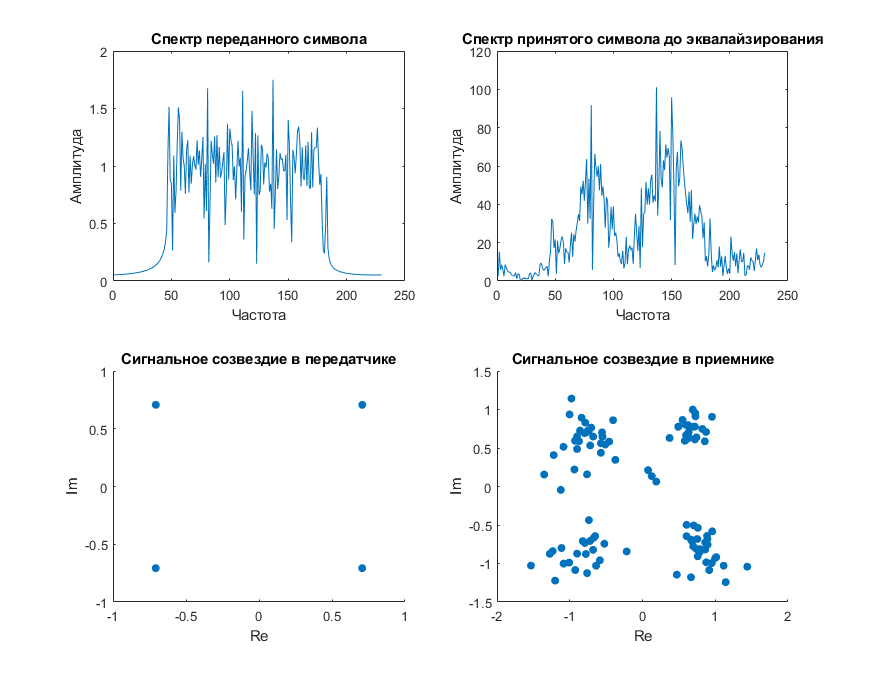
\includegraphics[width=\textwidth]{spectrum_const.png}
    \caption{Результаты моделирования}
    \label{fig:results}
\end{figure}
Рисунок \ref{fig:results} демонстрирует спектры переданного и принятого сигналов, а также сигнальные созвездия до и после передачи через канал. Спектр принятого сигнала демонстрирует влияние многолучевости и шума. Сигнальное созвездие в приемнике показывает, как шум и искажения канала влияют на расположение принятых символов по сравнению с идеальным созвездием на передатчике. Наличие ошибок (BER > 0) подтверждает влияние канала на качество передачи.

\chapter*{Заключение}
\addcontentsline{toc}{chapter}{Заключение}

В результате выполнения цикла практических работ была реализована полная модель системы цифровой связи. В процессе выполнения задач были освоены и применены следующие основные блоки и технологии:
\begin{itemize}
    \item \textbf{Кодирование источника}: Преобразование текстовой информации в битовую последовательность и обратное преобразование.
    \item \textbf{Помехоустойчивое кодирование}: Использование сверточного кодера и декодера Витерби для защиты информации от ошибок.
    \textbf{Перемежение}: Применение перемежителя для преобразования пакетных ошибок в случайные.
    \item \textbf{QPSK модуляция}: Отображение битовой последовательности в комплексные символы для передачи по каналу.
    \item \textbf{OFDM модуляция}: Формирование OFDM символа с пилотными символами, нулевыми поднесущими и циклическим префиксом.
    \item \textbf{Модель канала с замираниями и шумом}: Моделирование реальных условий распространения сигнала с учетом многолучевости и АБГШ.
    \item \textbf{Демодуляция и декодирование}: Восстановление исходных данных из принятого сигнала, включая OFDM демодуляцию, эквалайзирование, QPSK демодуляцию, деперемежение и декодирование Витерби.
\end{itemize}
В ходе тестирования была продемонстрирована работоспособность каждого из реализованных блоков, а также всей системы в целом. Расчет BER и построение графиков позволили оценить влияние модельного канала на качество передачи и увидеть эффект помехоустойчивого кодирования и эквалайзирования.

Полученные результаты показывают, что реализованная система способна передавать информацию через модельный канал.                                     % Вторая глава
\chapter{Знаковое кодирование}

\section{Введение}

Знаковое кодирование представляет собой метод представления текстовой информации в двоичном формате. Основная цель этой практической работы – реализовать процесс кодирования и декодирования текстового сообщения, используя заданный алфавит и разрядность кодового слова.

\section{Описание знакового кодера}

Знаковый кодер предназначен для преобразования входного символьного сообщения в последовательность двоичных символов (бит). Исходное сообщение состоит из латинских букв (маленьких и заглавных), цифр (0–9), пробела и точки, всего 64 символа.

\subsection{Принцип работы кодера}

Каждому символу входного сообщения присваивается уникальный двоичный код.

Количество бит для кодирования одного символа определяется разрядностью кодового слова.

Итоговое битовое сообщение формируется путем последовательного соединения кодов всех символов исходного текста.

\subsection{Описание входных и выходных данных}

Входные данные: текстовое сообщение длиной от 30 до 100 символов.

Выходные данные: битовая последовательность, представляющая закодированное сообщение.

\section{Описание знакового декодера}

Знаковый декодер выполняет обратную операцию: преобразует битовую последовательность обратно в текстовое сообщение. Для этого используется та же знаковая кодировка, что и в кодере.

\subsection{Принцип работы декодера}

Битовое сообщение разделяется на фрагменты, соответствующие длине кодового слова.

Каждому фрагменту сопоставляется соответствующий символ из заданного алфавита.

Восстанавливается исходное текстовое сообщение.

\subsection{Описание входных и выходных данных}

Входные данные: битовая последовательность.

Выходные данные: исходное текстовое сообщение.

\section{Выводы}

В данной работе был рассмотрен процесс знакового кодирования и декодирования текстового сообщения. Реализованный кодер позволяет эффективно преобразовывать текст в битовую форму, а декодер успешно восстанавливает исходные данные. Этот метод широко применяется в системах обработки и хранения информации.
\chapter{Формирование и передача OFDM сигнала}

\section{Практика 5. OFDM модуляция}

\subsection{Описание}
Пятая практическая работа посвящена реализации модуляции по принципу OFDM (Orthogonal Frequency-Division Multiplexing - ортогональное частотное мультиплексирование). OFDM является широко используемым методом модуляции в современных системах связи благодаря своей устойчивости к многолучевому распространению и интерференции.

\subsection{Реализация}
Был разработан OFDM модулятор (\texttt{ofdm\_modulator.m}) со следующими ключевыми компонентами:
\begin{itemize}
    \item \textbf{Вставка пилотных символов}: В сигнал добавляются известные пилотные символы для последующей оценки канала.
    \item \textbf{Добавление нулевых поднесущих}: Добавляются нулевые поднесущие по краям спектра для обеспечения защиты от внеполосных излучений и облегчения фильтрации.
    \item \textbf{Применение ОБПФ}: Выполняется обратное быстрое преобразование Фурье для формирования временного OFDM символа.
    \item \textbf{Добавление циклического префикса}: В начало OFDM символа добавляется копия его конца для борьбы с межсимвольной интерференцией.
\end{itemize}
Параметры модуляции, такие как интервал пилотных символов ($\Delta R_s$), длина циклического префикса ($T_{CP}$), процент нулевых поднесущих ($C$) и общее число поднесущих ($N_{subcarrier}$), сохраняются для использования в демодуляторе.

\subsection{Результаты тестирования}
В данной практической работе производится только модуляция, без обратного преобразования. Проверка корректности производится на последующих этапах, когда сигнал пройдет через канал и будет демодулирован. Консольный вывод показывает фрагмент сгенерированного OFDM символа.

\begin{verbatim}
% START - TASK: 5
disp('TASK 5: ');

delta_Rs = 6;
T_CP = 16;
C = 0.25;
N_subcarrier = 128;

ofdm_symbol = ofdm_modulator(modulatedSymbols, delta_Rs, T_CP, C, N_subcarrier);

% disp(ofdm_symbol) % Полный вывод закомментирован в коде

% END - TASK: 5
\end{verbatim}

\subsection{Консольный вывод}
\begin{verbatim}
TASK 5:
\end{verbatim}
(Консольный вывод для этой задачи пустой, так как \texttt{disp(ofdm\_symbol)} закомментировано)

\section{Практика 6. Модель канала передачи}

\subsection{Описание}
Шестая практическая работа посвящена реализации модели канала передачи с учетом замираний и аддитивного белого гауссовского шума (АБГШ). Реалистичная модель канала необходима для оценки производительности системы связи в условиях, приближенных к реальным.

\subsection{Реализация}
Была реализована функция \texttt{channel\_model.m}, моделирующая канал со следующими характеристиками:
\begin{itemize}
    \item \textbf{Многолучевое распространение}: Сигнал достигает приемника по нескольким путям ($N_b$ лучей) с разными задержками и ослаблениями.
    \item \textbf{Случайные задержки лучей}: Задержки для каждого луча генерируются случайным образом.
    \item \textbf{Добавление АБГШ}: К сигналу примешивается аддитивный белый гауссовский шум с заданной мощностью ($N_0$), определяемой отношением сигнал/шум (SNR).
\end{itemize}
Модель канала принимает на вход OFDM символ и возвращает принятый сигнал, прошедший через канал.

\subsection{Результаты тестирования}
Работа модели канала была проверена путем пропускания OFDM символа, сгенерированного на предыдущем этапе, через модель. Консольный вывод показывает фрагмент принятого сигнала.

\begin{verbatim}
% START - TASK: 6
disp('TASK 6: ');

N_path = 3;
N0_dB = 15;
max_delay = 6;
rx_signal = channel_model(ofdm_symbol, N_path, N0_dB, max_delay);

disp(rx_signal); % Отображение полного сигнала
% END - TASK: 6
\end{verbatim}

\subsection{Консольный вывод}
\begin{verbatim}
TASK 6:
  Columns 1 through 13

   1.3812 - 0.8223i   0.0111 - 0.1080i  -1.0138 + 0.7830i ... (фрагмент)

  Columns 14 through 26

   0.7438 - 1.3265i  -3.3089 + 0.5977i   1.1598 + 0.3892i ... (фрагмент)

  Columns ... (и так далее для всех столбцов)

   ...  0.0007 + 0.0138i
\end{verbatim}
Принятый сигнал представляет собой комплексные значения, которые включают в себя искажения от канала и шум. В документе представлен только фрагмент для наглядности.

\section{Практика 7. Эквалайзирование и OFDM демодуляция}

\subsection{Описание}
Седьмая практическая работа посвящена реализации приемной части системы связи, включающей OFDM демодуляцию и эквалайзирование. Эти этапы позволяют восстановить исходные символы из принятого OFDM сигнала, прошедшего через канал.

\subsection{Реализация}
Был разработан OFDM демодулятор (\texttt{ofdm\_demodulator.m}), выполняющий следующие действия:
\begin{itemize}
    \item \textbf{Удаление циклического префикса}: Удаляется добавленный на передаче циклический префикс.
    \item \textbf{БПФ}: Выполняется быстрое преобразование Фурье для перехода из временной области в частотную.
    \item \textbf{Оценка канала по пилотным символам}: Используются принятые пилотные символы для оценки частотной характеристики канала.
    \item \textbf{Эквалайзирование}: Выполняется компенсация искажений, внесенных каналом, на основе оценки канала.
    \item \textbf{Удаление нулевых поднесущих}: Удаляются нулевые поднесущие, добавленные на передаче.
\end{itemize}
Полученные в результате демодуляции символы (QPSK символы) далее передаются на демодулятор QPSK.

\subsection{Результаты тестирования}
Корректность работы OFDM демодулятора и эквалайзера оценивается на следующем этапе, где происходит демодуляция полученных символов и декодирование битовой последовательности.

\begin{verbatim}
% START - TASK: 7

disp('TASK 7: ');

received_symbols = ofdm_demodulator(rx_signal, delta_Rs, T_CP, C, N_subcarrier);
% received_symbols = ofdm_demodulator(ofdm_symbol, delta_Rs, T_CP, C, N_subcarrier);
demodulatedBits = qpsk_demodulator(received_symbols);

% disp('Original QPSK symbols:'); % Полный вывод закомментирован
% disp(modulatedSymbols);
% disp('Received QPSK symbols:'); % Полный вывод закомментирован
% disp(received_symbols);

% END - TASK: 7
\end{verbatim}

\subsection{Консольный вывод}
\begin{verbatim}
TASK 7:
\end{verbatim}
(Консольный вывод для этой задачи пустой)

\section{Практика 8. Расчет характеристик и построение графиков}

\subsection{Описание}
Восьмая практическая работа посвящена анализу производительности разработанной системы связи путем расчета коэффициента битовых ошибок (BER) и построения графиков, иллюстрирующих спектр сигналов и сигнальные созвездия.

\subsection{Реализация}
\subsubsection{Расчет BER}
Производится сравнение принятой и демодулированной битовой последовательности с исходной битовой последовательностью, полученной после перемежения. Подсчитывается количество ошибочных битов и вычисляется BER как отношение количества ошибок к общему числу переданных битов.

\subsubsection{Построение графиков}
Строятся следующие графики:
\begin{itemize}
    \item Спектр переданного OFDM символа.
    \item Спектр принятого OFDM символа (до эквалайзирования).
    \item Сигнальное созвездие QPSK символов в передатчике.
    \item Сигнальное созвездие QPSK символов в приемнике (после OFDM демодуляции и эквалайзирования).
\end{itemize}
Эти графики позволяют визуально оценить влияние канала на сигнал и эффективность эквалайзирования.

\subsection{Результаты тестирования}
Ниже представлены консольный вывод с рассчитанным BER и сгенерированные графики.

\begin{verbatim}
% START - TASK: 8
disp('TASK 8: ');

min_length = min(length(demodulatedBits), length(interleavedBits));

demodulatedBits_truncated = demodulatedBits(1:min_length);
interleavedBits_truncated = interleavedBits(1:min_length);

% Расчет BER
bit_errors = sum(demodulatedBits_truncated ~= interleavedBits_truncated);
total_bits = length(demodulatedBits_truncated);
BER = bit_errors / total_bits;

disp(['Количество ошибочных битов: ', num2str(bit_errors)]);
disp(['Общее количество битов: ', num2str(total_bits)]);
disp(['BER: ', num2str(BER)]);

figure(1);

subplot(2, 2, 1);
plot(abs(fft(ofdm_symbol)));
title('Спектр переданного символа');
xlabel('Частота');
ylabel('Амплитуда');

subplot(2, 2, 2);
plot(abs(fft(rx_signal)));
title('Спектр принятого символа до эквалайзирования');
xlabel('Частота');
ylabel('Амплитуда');

subplot(2, 2, 3);
scatter(real(modulatedSymbols), imag(modulatedSymbols), 'filled')
title('Сигнальное созвездие в передатчике');
xlabel('Re');
ylabel('Im');

subplot(2, 2, 4);
scatter(real(received_symbols), imag(received_symbols), 'filled');
title('Сигнальное созвездие в приемнике');
xlabel('Re');
ylabel('Im');

% END - TASK: 8
\end{verbatim}

\subsection{Консольный вывод}
\begin{verbatim}
TASK 8:
Количество ошибочных битов: 1
Общее количество битов: 204
BER: 0.004902
\end{verbatim}

\subsection{Графические результаты}
\begin{figure}[h!]
    \centering
    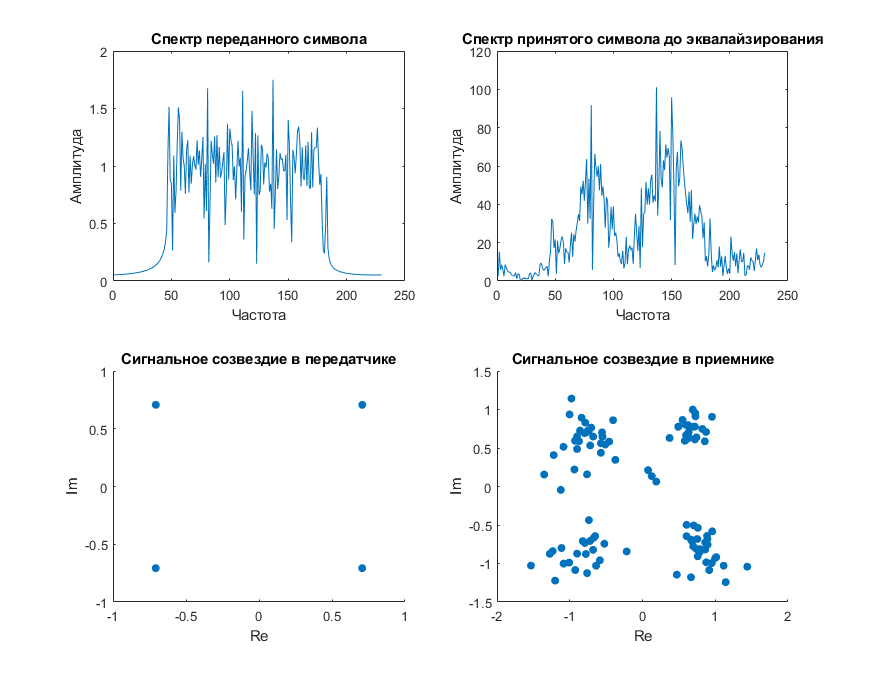
\includegraphics[width=\textwidth]{spectrum_const.png}
    \caption{Результаты моделирования}
    \label{fig:results}
\end{figure}
Рисунок \ref{fig:results} демонстрирует спектры переданного и принятого сигналов, а также сигнальные созвездия до и после передачи через канал. Спектр принятого сигнала демонстрирует влияние многолучевости и шума. Сигнальное созвездие в приемнике показывает, как шум и искажения канала влияют на расположение принятых символов по сравнению с идеальным созвездием на передатчике. Наличие ошибок (BER > 0) подтверждает влияние канала на качество передачи.

\chapter*{Заключение}
\addcontentsline{toc}{chapter}{Заключение}

В результате выполнения цикла практических работ была реализована полная модель системы цифровой связи. В процессе выполнения задач были освоены и применены следующие основные блоки и технологии:
\begin{itemize}
    \item \textbf{Кодирование источника}: Преобразование текстовой информации в битовую последовательность и обратное преобразование.
    \item \textbf{Помехоустойчивое кодирование}: Использование сверточного кодера и декодера Витерби для защиты информации от ошибок.
    \textbf{Перемежение}: Применение перемежителя для преобразования пакетных ошибок в случайные.
    \item \textbf{QPSK модуляция}: Отображение битовой последовательности в комплексные символы для передачи по каналу.
    \item \textbf{OFDM модуляция}: Формирование OFDM символа с пилотными символами, нулевыми поднесущими и циклическим префиксом.
    \item \textbf{Модель канала с замираниями и шумом}: Моделирование реальных условий распространения сигнала с учетом многолучевости и АБГШ.
    \item \textbf{Демодуляция и декодирование}: Восстановление исходных данных из принятого сигнала, включая OFDM демодуляцию, эквалайзирование, QPSK демодуляцию, деперемежение и декодирование Витерби.
\end{itemize}
В ходе тестирования была продемонстрирована работоспособность каждого из реализованных блоков, а также всей системы в целом. Расчет BER и построение графиков позволили оценить влияние модельного канала на качество передачи и увидеть эффект помехоустойчивого кодирования и эквалайзирования.

Полученные результаты показывают, что реализованная система способна передавать информацию через модельный канал.

% \chapter{Таблицы}
\label{ch:tab}
    Наконец, разберемся с таблицами. В принципе, \LaTeX{} позволяет делать большие и сложные таблицы, но вручную обычно их не пишут; для этого используют разные сайты типа \href{https://www.tablesgenerator.com/}{типа такого}. По ГОСТ заморачиваться с таблицами особо не надо, главное чтобы правильно были заданы подписи, работала нумерация и ссылки. Все необходимые стилевые условия уже зашиты в данный шаблон. Помните, что в конце заголовка таблицы, как и в конце подписи к рисунку, точка не ставится! Воспользовавишись сайтом по данной выше ссылке, можем сделать, например, такую таблицу:
\begin{table}[ht]
\caption{Вот так выглядит рандомная таблица из Интернета с ценой разных животных, которых можно найти в мире}
\label{tab:t1}
\centering
\begin{tabular}{llr}
\hline
Animal    & Description & Price (\$) \\ \hline
Gnat      & per gram    & 13.65      \\
          & each        & 0.01       \\
Gnu       & stuffed     & 92.50      \\
Emu       & stuffed     & 33.33      \\
Armadillo & frozen      & 8.99       \\ \hline
\end{tabular}
\end{table}

На эту таблицу, безусловно, можно так же ссылаться. Давайте сошлемся на \hyperref[tab:t1]{Таблицу \ref*{tab:t1}} и на этом, пожалуй, закончим.

\endinput                                     % Третья глава
% \chapter{Графики}
\label{ch:plot}

Краткое описанике по построению графиков при помощи PGFPlots \cite{habrpgfplots}.

	% \begin{figure}[ht]
    %     \centering
	% 	\begin{tikzpicture}
	% 		\begin{axis} [
	% 			legend pos = north west, 
	% 			ymin = 0, 
	% 			grid = major
	% 		]
	% 		\legend{ 
	% 			$\log_2(x)$, 
	% 			$\ln(x)$, 
	% 			$\log_{10}(x)$
	% 		};
	% 		\addplot {log2(x)};
	% 		\addplot {ln(x)};
	% 		\addplot {log10(x)};
	% 		\end{axis}
	% 	\end{tikzpicture}
	% 	\caption{Простая подпись к графикам}\label{}
	% \end{figure}

А здесь будет продолжение текста.
\endinput                                     % Четвертая глава



% \printbibliography[title=Список использованных источников] % Автособираемый список литературы

\end{document}